% \iffalse
\let\negmedspace\undefined
\let\negthickspace\undefined
\documentclass[journal,12pt,twocolumn]{IEEEtran}
\usepackage{cite}
\usepackage{amsmath,amssymb,amsfonts,amsthm}
\usepackage{algorithmic}
\usepackage{graphicx}
\usepackage{textcomp}
\usepackage{xcolor}
\usepackage{txfonts}
\usepackage{listings}
\usepackage{enumitem}
\usepackage{mathtools}
\usepackage{float}
\usepackage{gensymb}
\usepackage{comment}
\usepackage[breaklinks=true]{hyperref}
\usepackage{tkz-euclide} 
\usepackage{listings}
\usepackage{gvv}                                        
\def\inputGnumericTable{}                                 
\usepackage[latin1]{inputenc}                                
\usepackage{color}                                            
\usepackage{array}                                            
\usepackage{longtable}                                       
\usepackage{calc}                                             
\usepackage{multirow}                                         
\usepackage{hhline}                                           
\usepackage{ifthen}                                           
\usepackage{lscape}
\usepackage{amsmath}
\newtheorem{theorem}{Theorem}[section]
\newtheorem{problem}{Problem}
\newtheorem{proposition}{Proposition}[section]
\newtheorem{lemma}{Lemma}[section]
\newtheorem{corollary}[theorem]{Corollary}
\newtheorem{example}{Example}[section]
\newtheorem{definition}[problem]{Definition}
\newcommand{\BEQA}{\begin{eqnarray}}
\newcommand{\EEQA}{\end{eqnarray}}
\newcommand{\define}{\stackrel{\triangle}{=}}
\theoremstyle{remark}
\newtheorem{rem}{Remark}
\begin{document}

\bibliographystyle{IEEEtran}
\title{NCERT 11.9.1.13Q}
\author{EE23BTECH11015 - DHANUSH V NAYAK$^{*}$% <-this % stops a space
}
\maketitle
\newpage
\bigskip
\renewcommand{\thefigure}{\arabic{figure}}
\renewcommand{\thetable}{\theenumi}
\textbf{Question:} Write the first five terms of each of the sequences in Exercises 11 to 13 and obtain the corresponding series:\\
$a_1=a_2=2,$\hspace{5pt} $a_n=a_{n-1} -1,$\hspace{5pt} $n>2$\\
\textbf{Solution:}
\begin{table}[H]
\centering
\renewcommand\thetable{1}
\setlength{\extrarowheight}{9pt}
\resizebox{0.5\textwidth}{!}{
\begin{tabular}{|c|c|c|}
\hline
\textbf{Parameter} & \textbf{Description} & \textbf{Value} \\ \hline
$x\brak{0}$ & First term &2 \\ \hline
$x\brak{1}$ & Second term &2 \\ \hline
ROC & Region of convergence & $\left\{ z : \left|\sum_{n=-\infty}^{\infty} x(n)z^{-n}\right| < \infty \vphantom {\brak{{0.3pt}}}\right\}$ \\ \hline 
$x_h\brak{n}$ & Homogenous solution & --- \\ \hline
$x_t\brak{n}$ & Transient solution & ---\\ \hline
\end{tabular}}
\caption{Parameter Table}
\label{tab:11.9.1.13}
\end{table}

\begin{align}
    x\brak{n+1} - x\brak{n} &= -u\brak{n-1} , n\geq 0 \label{eq:11.9.1.13.1}
\end{align}
Homogeneous solution :-
\begin{align}
    x\brak{n+1} - x\brak{n} &= 0\\
    x_h\brak{n} &= cu\brak{n}
\end{align}
From table \ref{tab:11.9.1.13}
\begin{align}
    x\brak{0} &= 2\\
    \therefore c&=2\\
    x_h\brak{n} &= 2u\brak{n}
\end{align}
Transient solution :
\begin{align}
     x\brak{n+1} - x\brak{n} &= -u\brak{n-1} \label{eq:transient_equation}
\end{align}
One sided $Z$-transform is defined as :
\begin{align}
    X\brak{z} &= \sum_{n=0}^\infty x\brak{n} z^{-n}
\end{align}
Time shifting property :
\begin{align}
	x\brak{n-k}&\system{Z} z^{-k}X\brak{z}\label{eq:shiftk}\\
\implies x\brak{n+1} &\system{Z} z\brak{X\brak{z}} \label{eq:11.9.1.13.2} \\
\implies u\brak{n-1} &\system{Z} \frac{z^{-1}}{1-z^{-1}} \label{eq:11.9.1.13.3}
\end{align}
Applying one-sided $Z$-transform on equation\eqref{eq:transient_equation} and using results of equation\eqref{eq:11.9.1.13.2} and \eqref{eq:11.9.1.13.3}
\begin{align}
    z\brak{X\brak{z}}- X\brak{z} &= -\frac{z^{-1}}{1-z^{-1}}
\end{align}
\begin{align}
    X\brak{z} &= \frac{z^{-2}}{\brak{1-z^{-1}}^2}  ,   \abs{z} >1\label{eq:11.9.1.13.4}
\end{align}
Substituting result of equation \eqref{eq:11.9.5.26.9}  in equation \eqref{eq:11.9.1.13.4}:
\begin{align}
    x_t\brak{n} &= \brak{1-n}u\brak{n-1}
\end{align}
Now,
\begin{align}
    x\brak{n} &= x_h\brak{n} + x_t\brak{n} \\
                &= 2u\brak{n} + \brak{1-n}u\brak{n-1}
\end{align} 
\begin{figure}[htbp]
    \centering
    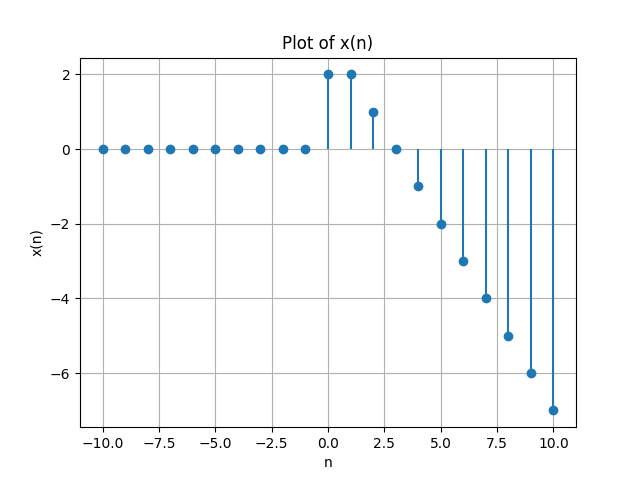
\includegraphics[width=1\columnwidth]{figs/fig_x(n).png}
    \caption{Stem Plot of $x\brak{n}$}
    \label{fig:x(n)}
\end{figure}
\end{document}
